%%%%%%%%%%%%%%%%%%%%%%%%%%%%%%%%%%%%%%%%%%%%%%%%%%%%%%%%%%%%%%%%%%%%%%%%%%%%%%%%%%%%%%%%%%%%%%%%%%%%%%%%%%%%%%%%%%%%%%%%%
\subsection{Motivation}
%%%%%%%%%%%%%%%%%%%%%%%%%%%%%%%%%%%%%%%%%%%%%%%%%%%%%%%%%%%%%%%%%%%%%%%%%%%%%%%%%%%%%%%%%%%%%%%%%%%%%%%%%%%%%%%%%%%%%%%%%

%%%%%%%%%%%%%%%%%%%%%%%%%%%%%%%%%%%%%%%%%%%%%%%%%%%%%%%%%%%%%%%%%%%%%%%%%%%%%%%%%%%%%%%%%%%%%%%%%%%%%%%%%%%%%%%%%%%%%%%%%
\begin{frame}
\frametitle{Author Identification}

\begin{columns}
\column{0.5\textwidth}
% With the development of more complex robotic and intelligent systems, many now contain \textbf{several sensors, often of multiple modalities}

The problem of author identification has been extensively studied, which aims to learn a model to rank potential authors for an anonymous paper based on public information.

% \fullcite{DAA}

\pause
\begin{block}{Possible Uses}
    \begin{itemize}
        \item Author identification
        \item Relevance search
        \item Personalized recommendations
        \item Reviewer recommendation
        \item Collaboration discovery
    \end{itemize}
\end{block}

\column{0.5\textwidth}
\begin{center}
\begin{tabular}{c}
\onslide<1->
\includegraphics[width=\textwidth]{img/journals}
% 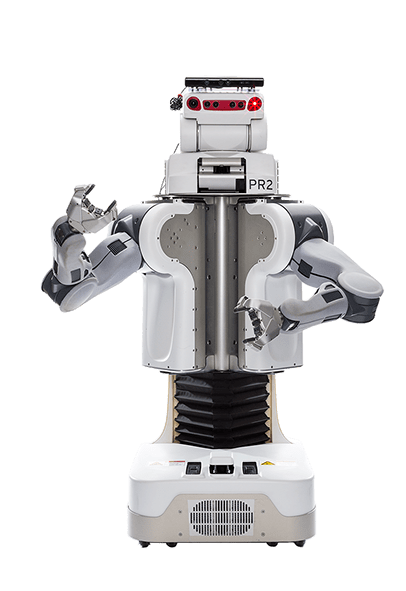
\includegraphics[width=0.8\textwidth]{img/pr2/pr2_a}
\end{tabular}
\end{center}
\end{columns}
\end{frame}
%%%%%%%%%%%%%%%%%%%%%%%%%%%%%%%%%%%%%%%%%%%%%%%%%%%%%%%%%%%%%%%%%%%%%%%%%%%%%%%%%%%%%%%%%%%%%%%%%%%%%%%%%%%%%%%%%%%%%%%%
\begin{frame}
\frametitle{Problem formulation}
\begin{columns}
\column{0.5\textwidth}

Current approaches:
\begin{itemize}
    \item Focus on single author identification
    \item Do not account for the optimal number of writers
    \item Do not take into account the relation between possible authors
\end{itemize}

\column{0.2\textwidth}
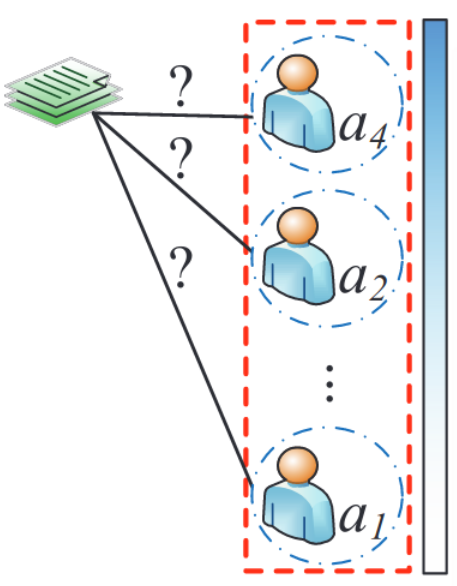
\includegraphics[width=1\linewidth]{img/single_author}
\column{0.3\textwidth}
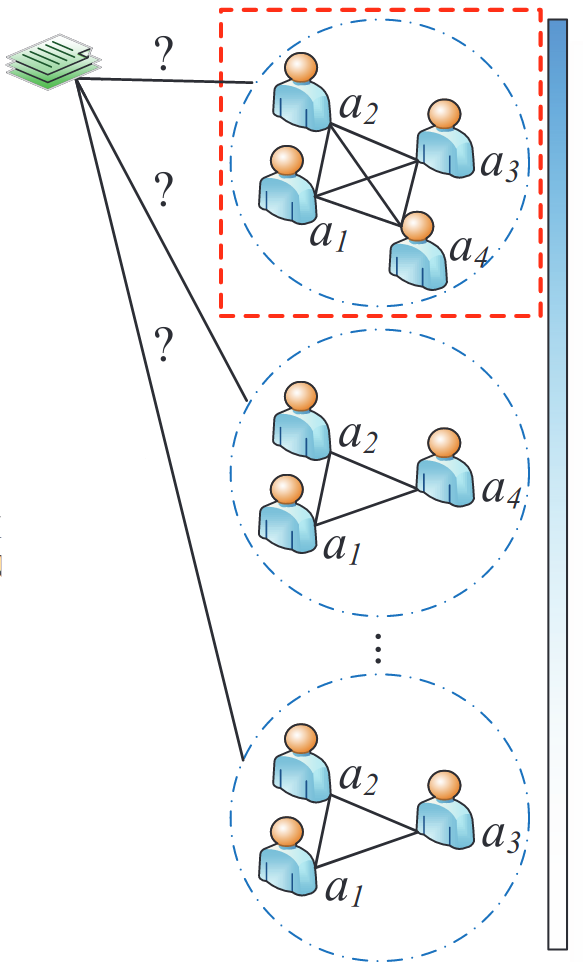
\includegraphics[width=1\linewidth]{img/multiple_author}


\end{columns}
\end{frame}
%%%%%%%%%%%%%%%%%%%%%%%%%%%%%%%%%%%%%%%%%%%%%%%%%%%%%%%%%%%%%%%%%%%%%%%%%%%%%%%%%%%%%%%%%%%%%%%%%%%%%%%%%%%%%%%%%%%%%%%%%
\subsection{Important Concepts}
%%%%%%%%%%%%%%%%%%%%%%%%%%%%%%%%%%%%%%%%%%%%%%%%%%%%%%%%%%%%%%%%%%%%%%%%%%%%%%%%%%%%%%%%%%%%%%%%%%%%%%%%%%%%%%%%%%%%%%%%
\begin{frame}
\frametitle{Heterogeneous Information Network (HIN)}
\begin{columns}
\column{0.5\textwidth}

\begin{itemize}
    \item Directed graph
    \item Nodes and edges have types
\end{itemize}

\column{0.5\textwidth}
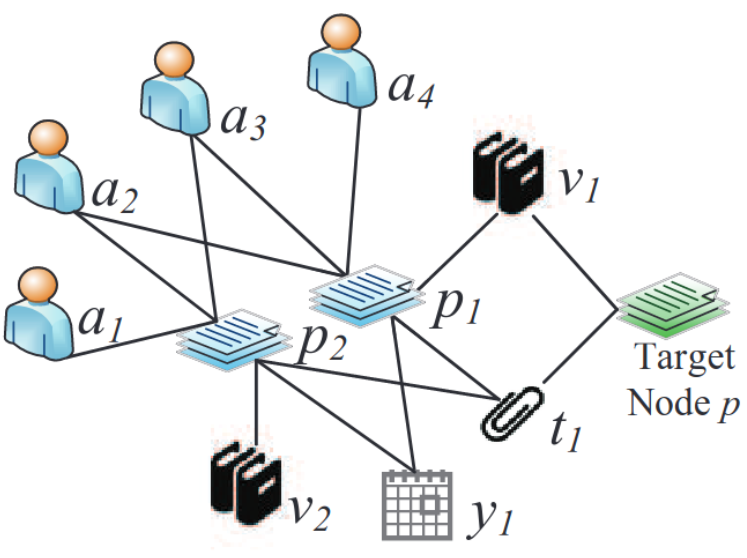
\includegraphics[width=1\linewidth]{img/hin}


\end{columns}
\end{frame}
%%%%%%%%%%%%%%%%%%%%%%%%%%%%%%%%%%%%%%%%%%%%%%%%%%%%%%%%%%%%%%%%%%%%%%%%%%%%%%%%%%%%%%%%%%%%%%%%%%%%%%%%%%%%%%%%%%%%%%%%
\begin{frame}
\frametitle{Clique (Graph Theory)}
\begin{columns}
\column{0.5\textwidth}

\begin{itemize}
    \item Undirected graph
    \item Subset of vertices such that every two distinct vertices are adjacent
\end{itemize}

\column{0.5\textwidth}
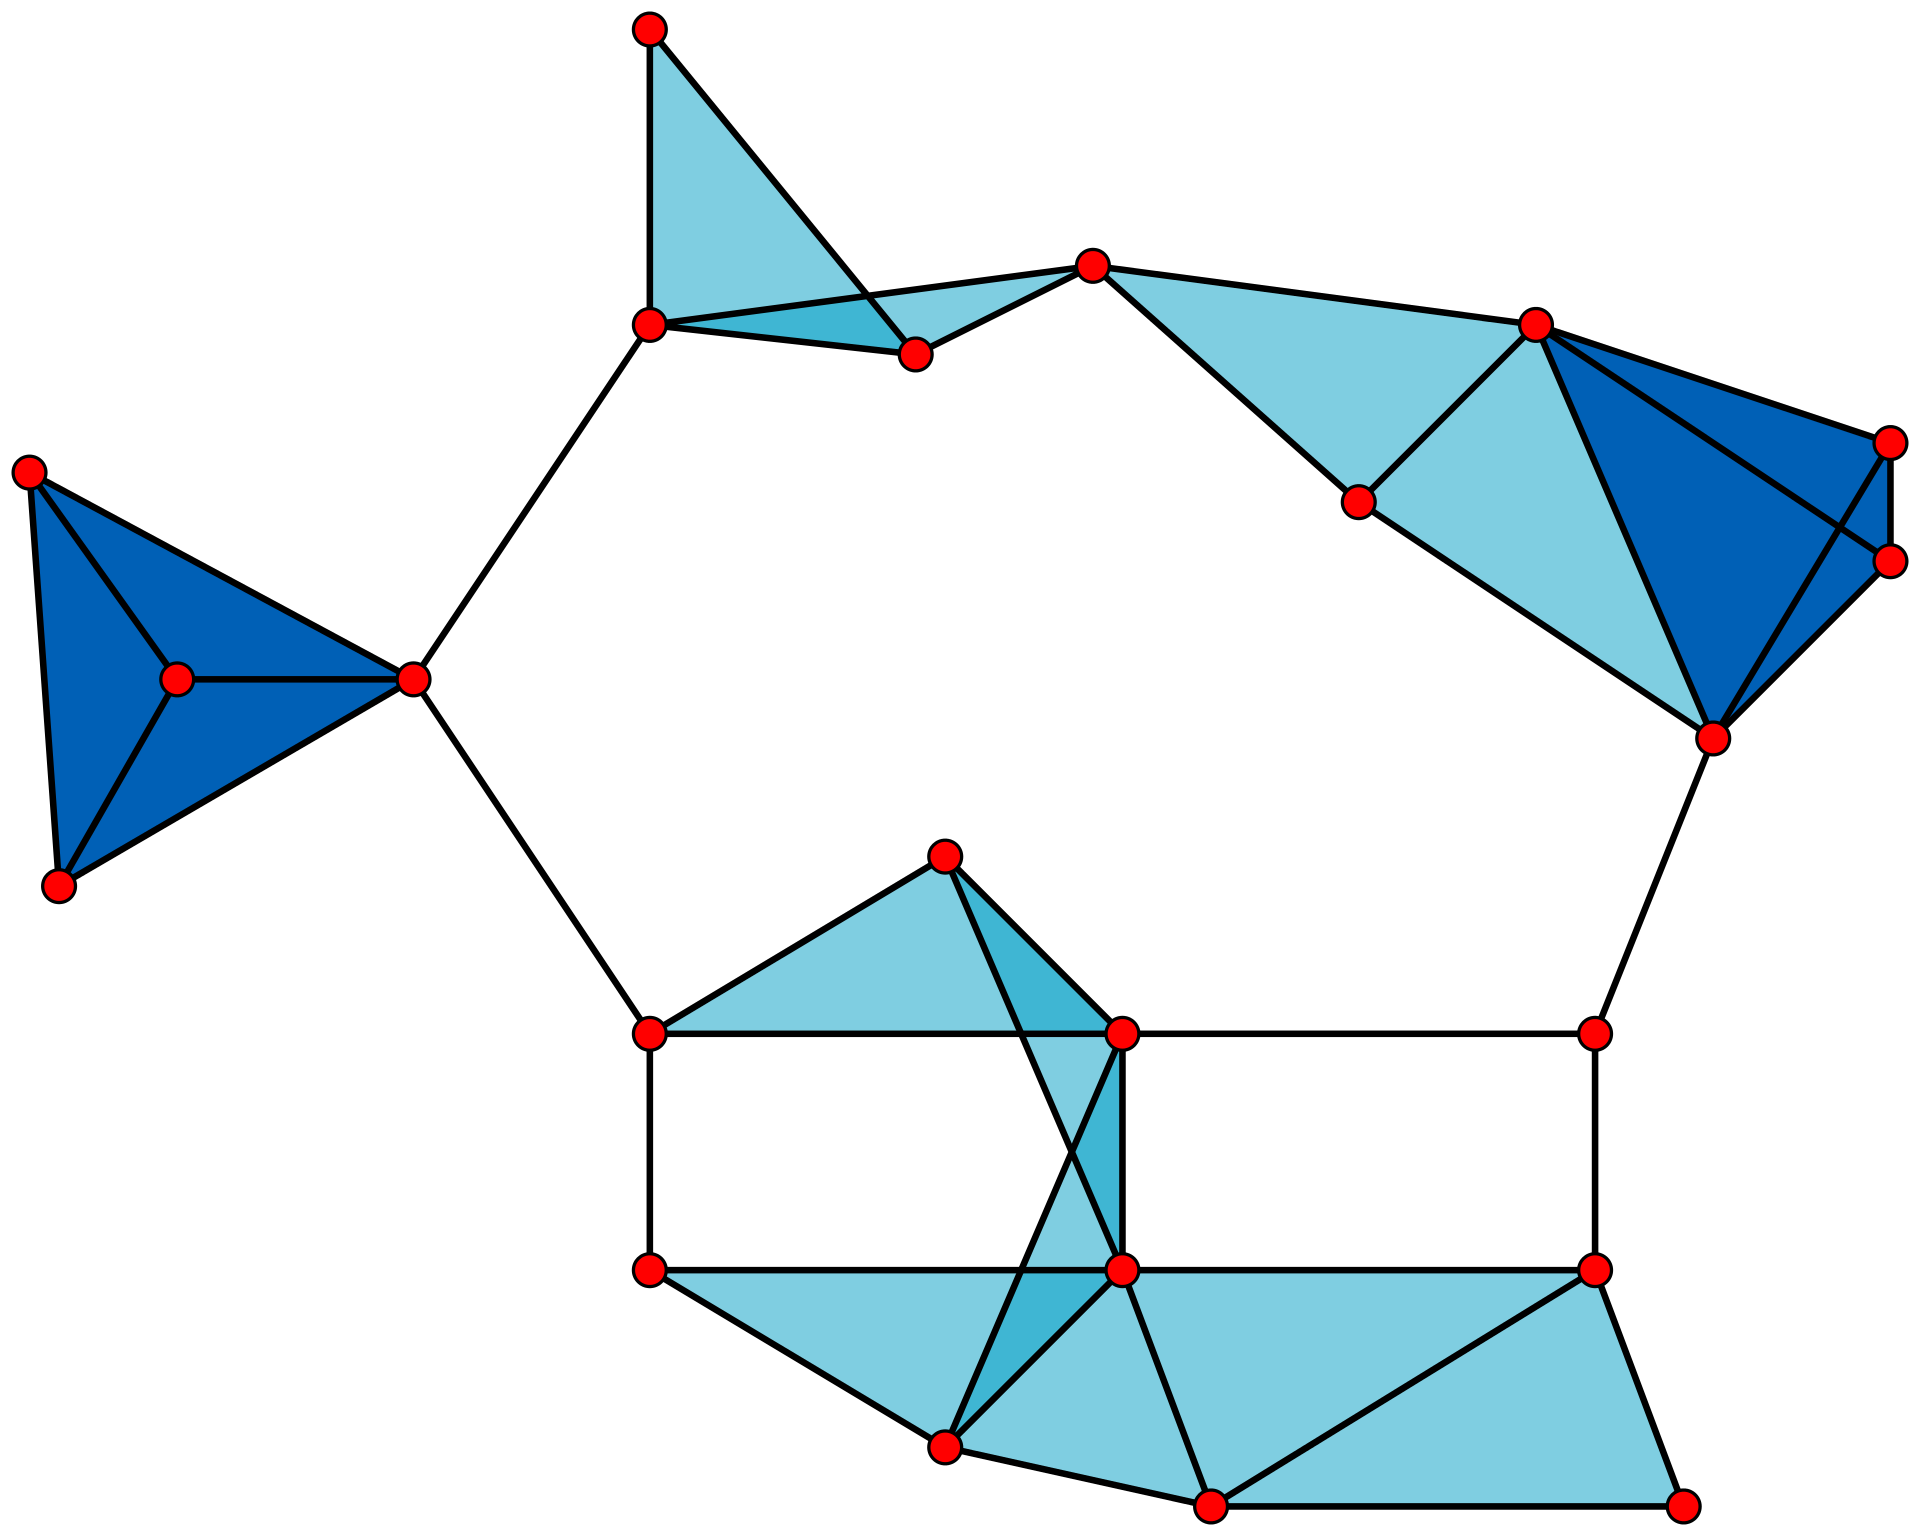
\includegraphics[width=1\linewidth]{img/clique}


\end{columns}
\end{frame}
%%%%%%%%%%%%%%%%%%%%%%%%%%%%%%%%%%%%%%%%%%%%%%%%%%%%%%%%%%%%%%%%%%%%%%%%%%%%%%%%%%%%%%%%%%%%%%%%%%%%%%%%%%%%%%%%%%%%%%%%
\begin{frame}
\frametitle{Quasi-Clique (Graph Theory)}
\begin{columns}
\column{0.5\textwidth}

A set of nodes S is an $\alpha$-quasi-clique if the edge density of the subgraph induced by S exceeds a threshold parameter $\alpha \in (0, 1)$

\column{0.5\textwidth}
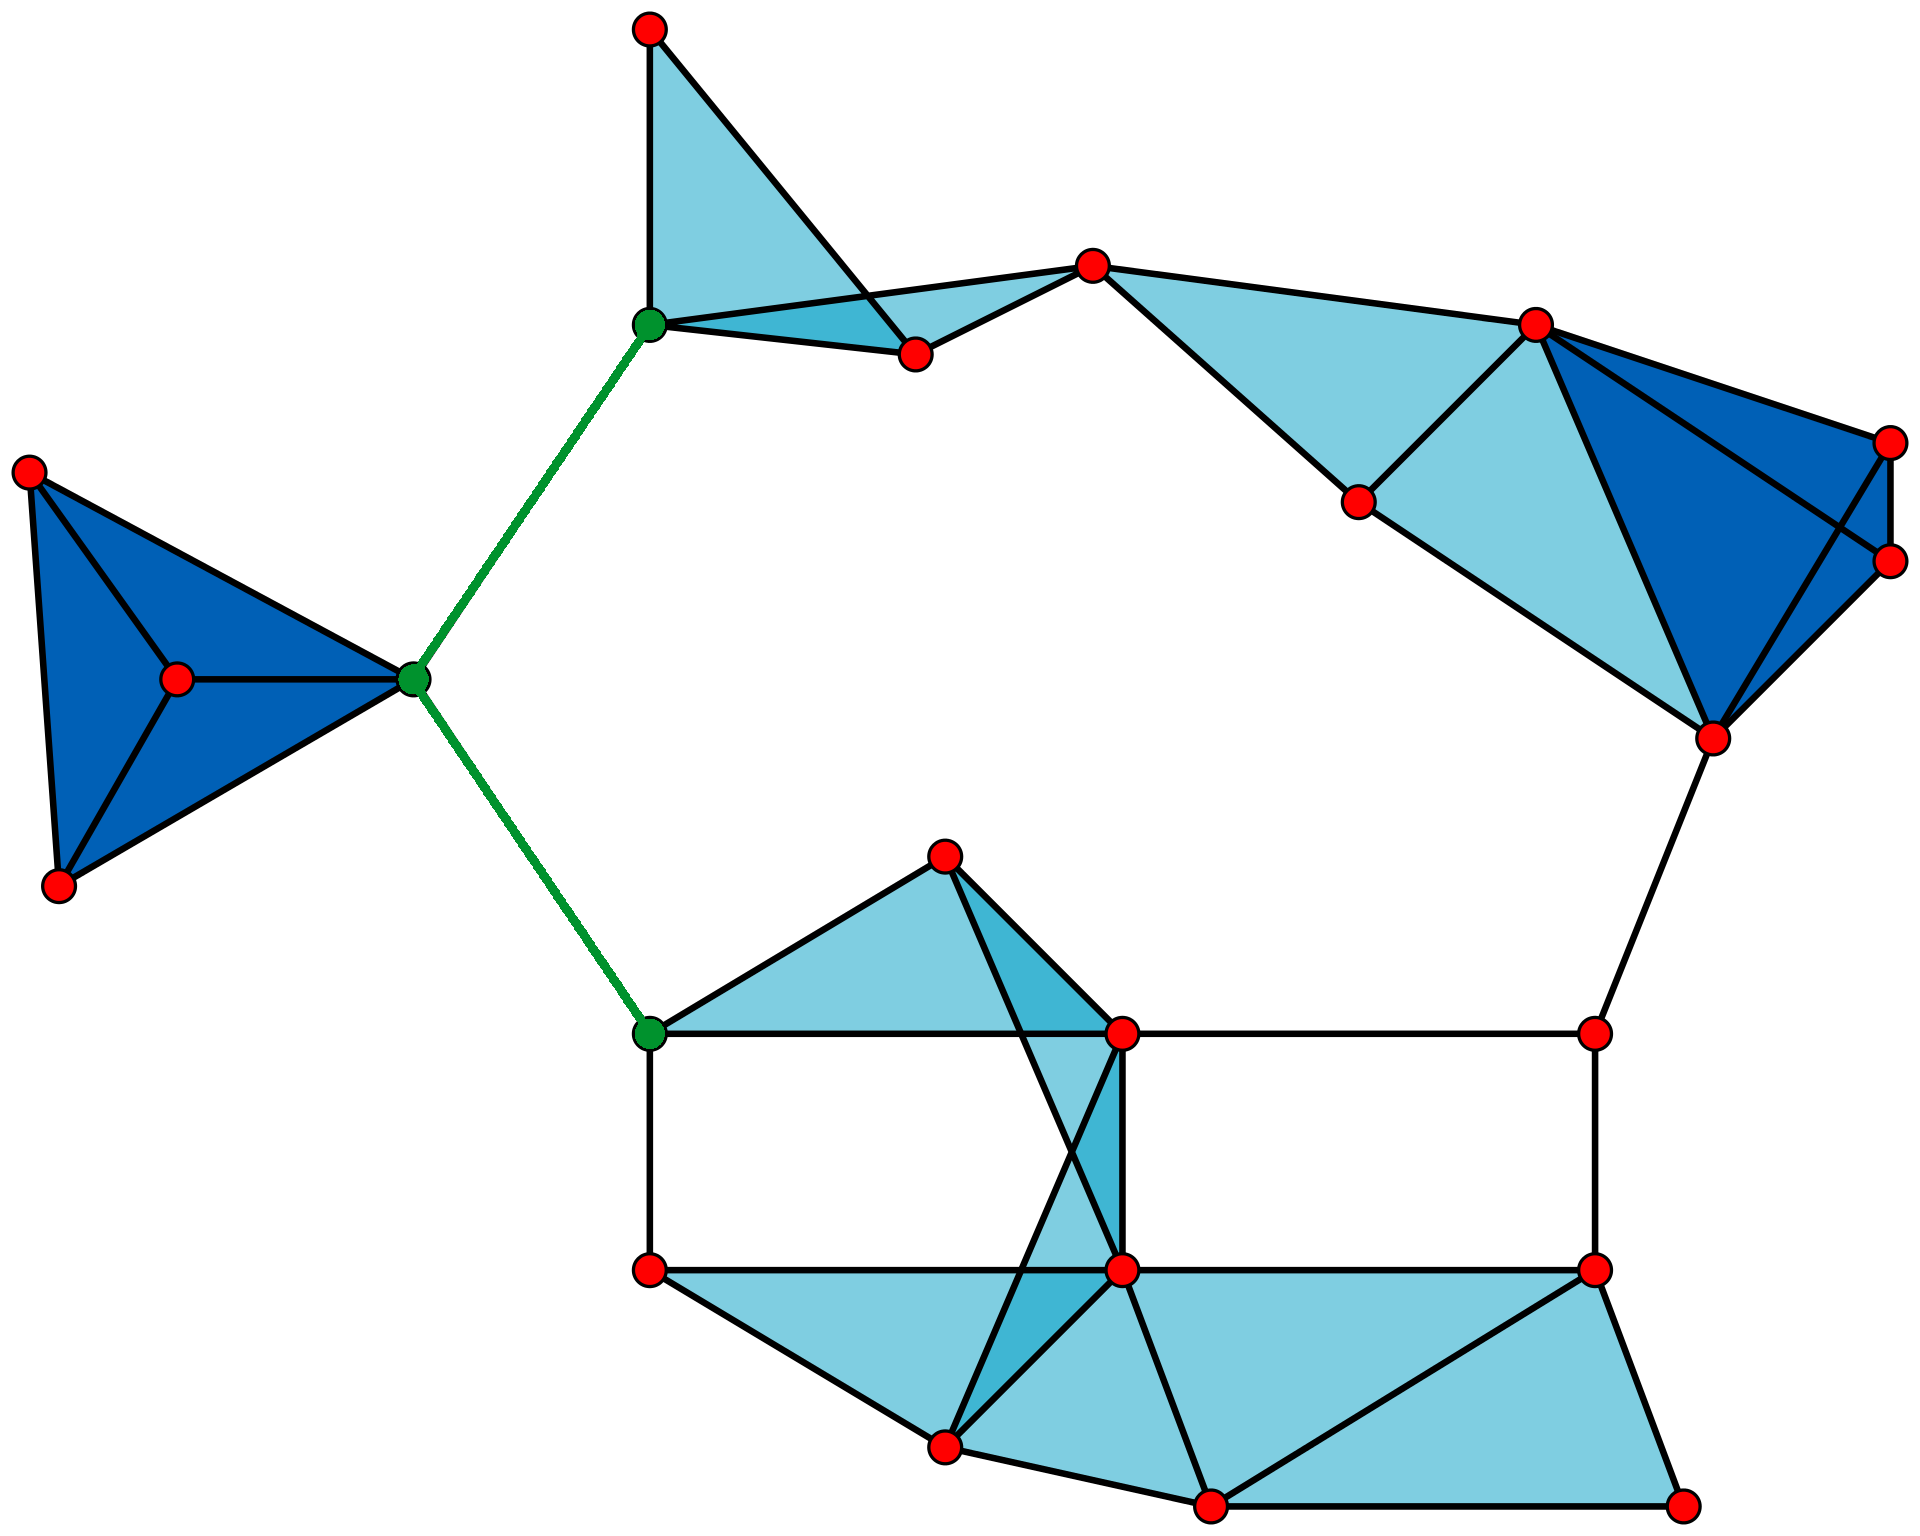
\includegraphics[width=1\linewidth]{img/quasi-clique}


\end{columns}
\end{frame}
%%%%%%%%%%%%%%%%%%%%%%%%%%%%%%%%%%%%%%%%%%%%%%%%%%%%%%%%%%%%%%%%%%%%%%%%%%%%%%%%%%%%%%%%%%%%%%%%%%%%%%%%%%%%%%%%%%%%%%%%